\subsection{Agile Modelle}
\label{sec:Kap-2.2.3}

\sttpLeserfuehrung{Bilder/Kapitel-2/Leserfuehrung/vorgehensmodelle_agile_illustration.pdf}{Bilder/Kapitel-2/Leserfuehrung/vorgehensmodelle_agile.pdf}

In den 1990er Jahren entstanden als Gegenbewegung zu den als schwergewichtig empfundenen vorherrschenden Softwareentwicklungsprozessen, die sich durch stark vorgegebene Abläufe und dokumentenorientierte Vorgehensweisen auszeichneten, sogenannte \textit{leichtgewichtige Modelle}. \marginline{leichtgewichtige Modelle}
Die Befürworter leichtgewichtiger Prozesse argumentierten, dass im Mittelpunkt von Softwareentwicklungsprojekten die Erstellung funktionierender Software und nicht die Abarbeitung von Regeln und das Produzieren von Dokumenten stehen müsse. Dementsprechend plädierten sie für eine Verschlankung und Flexibilisierung der Softwareentwicklungsprozesse. Basierend auf dieser Grundidee entwickelten sich Mitte bis Ende der 1990er Jahre die ersten leichtgewichtigen Vorgehensmodelle – wobei in diesem Kontext der Begriff 
\marginline{Entwicklungs\-modell}
\textit{Entwicklungsmodell} üblicher ist als Vorgehensmodell.

Die Bezeichnung \textbf{agil} für die leichtgewichtigen Modelle entstand, als sich im Februar 2001 in Utah, USA siebzehn Vertreter verschiedener leichtgewichtiger Modelle zu einem Gedankenaustausch versammelten, um Gemeinsamkeiten zwischen den verschiedenen Ansätzen zu finden. Alistair Cockburn, einer der Teilnehmer des Treffens, schrieb im Rückblick, dass der Begriff \textbf{leichtgewichtig} für viele Teilnehmer „eher eine Abneigung gegen etwas vermittelte als Vertrauen in etwas“ \cite[281]{coc03} und daher mit \textbf{agil} ein neuer Begriff gewählt wurde. Mit dieser Begriffswahl sollte zudem hervorgehoben werden, dass man im Laufe eines Softwareentwicklungsprojekts auf Veränderungen reagieren können muss. 

\sttpseitenrandzitat{„After a while we settled on Agile Software Development. Of course organizations would want to be agile. You can explain that to your CEO or customer far more easily than proclaiming you are extreme.“ \cite[16]{hun11}}{James Grenning, einer der Autoren des Agilen Manifests über die Wahl des Begriffs agil für Entwicklungsmethoden, die man bis dahin mit dem Extreme Programming verband.}

Auf  dem Treffen in Utah wurde als gemeinsame Erklärung das sogenannte 
\marginline{das Agile Manifest}
\textit{Agile Manifest} (Abb.~\ref{fig:das_agile_manifest}) verabschiedet. Es beinhaltet die grundlegende Philosophie der agilen Softwareentwicklung in Form von vier als \textit{Werte} bezeichneten Gegenüber\-stellungen. Wichtig ist, dass in diesem Manifest zwar eindeutige Präferenzen für die Aspekte in den ersten Satzhälften (\zb „Reagieren auf Veränderung“) zum Ausdruck gebracht werden, den Aspekten der zweiten Satzhälften (\zb „Befolgen eines Plans“), die dem Umfeld der schwergewichtigen Prozesse entstammen, aber ebenfalls Bedeutung beigemessen wird. So bedeutet zum Beispiel die Priorisierung funktionierender Software nicht zwingend den Verzicht auf eine (auch umfassendere) Dokumentation. Zusätzlich zu den Werten des Manifests einigten sich die Teilnehmer auf zwölf sogenannte \textit{Prinzipien}\footnote{\href{https://agilemanifesto.org/iso/de/principles.html}{https://agilemanifesto.org/iso/de/principles.html}.}, \marginline{Werte, Prinzipien}
die in Form von Handlungsanweisungen detaillierter als die Werte die Basis agiler Softwareentwicklung erläutern.

\begin{figure}[h!]
    \centering
    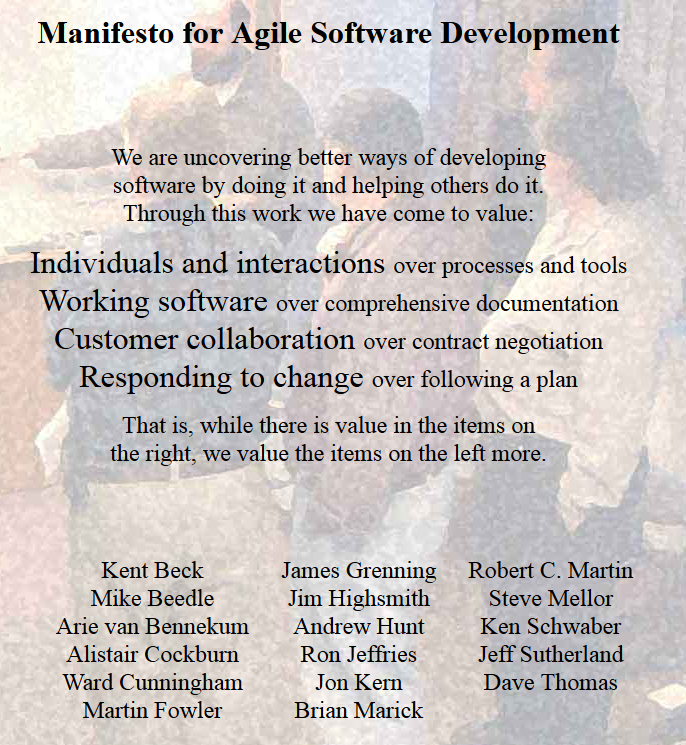
\includegraphics[scale=0.5]{Bilder/Kapitel-2/ScreenshotAgilesManifest.png}
    \caption[Das Agile Manifest]{Das Agile Manifest\\ (Screenshot von \href{https://agilemanifesto.org/iso/en/manifesto.html}{https://agilemanifesto.org/iso/en/manifesto.html})}
    \label{fig:das_agile_manifest}
\end{figure}

Mit der Verabschiedung des Agilen Manifests erfuhren die nun agil genannten Modelle einen – im zustimmenden wie im ablehnenden Sinne – enormen Bedeutungszuwachs. Werte und Prinzipien des Agilen Manifests bilden heute den Rahmen, innerhalb dessen sich – durchaus auch sehr verschiedenartige – Modelle und einzelne Methoden agil nennen. 

Agile Modelle sind immer iterative Modelle – allerdings nicht umgekehrt. Die iterative Entwicklung, in der für jede Produktversion alle Prozesse des Softwareengineering wiederholt durchlaufen werden, ist essentieller Bestandteil agiler Softwareentwicklung. Gleichzeitig sind agile Modelle auch inkrementelle Modelle, da es sich (ab einem gewissen Zeitpunkt im Projekt) zumindest bei Teilen der ausgelieferten Funktionalitäten um fertige Inkremente handelt, die nicht in späteren Versionen überarbeitet werden sollen.

\sttpHervorhebung{\textbf{Agile Modelle}} 
\marginline{Auslieferung}
\sttpHervorhebung{\textbf{liefern kontinuierlich lauffähige Software aus.}} 
Von einer ausgelieferten Produktversion zur nächsten vergehen in der Regel maximal einige Wochen. Aufgrund der kurzen Entwicklungszyklen spielen in agilen Modellen automatisiertes Testen, Verwendung existierender Frameworks und Bibliotheken sowie Einsatz von Entwicklungswerkzeugen eine besonders große Rolle. Erste Ideen und Ansätze, (Teile einer) Software schon während ihres laufenden Entwicklungsprozesses produktiv einzusetzen, hatte es bereits zu den Hochzeiten der Phasenmodelle in den 1980er Jahren gegeben \cite[84-2]{fav14}, aber erst im Kontext der agilen Modelle reiften diese Ideen zu einem grundlegenden Entwicklungsprinzip.

\sttpHervorhebung{\textbf{In agilen Modellen}} 
\marginline{Umgang mit Anforderungen} 
\sttpHervorhebung{\textbf{sind Anforderungsänderungen inhärenter Bestandteil des Softwareentwicklungsprozesses.}} 
Fehlende bzw. stark eingeschränkte Möglichkeiten auf die Änderung von Anforderungen zu reagieren, betrachten die Vertreter agiler Softwareentwicklung als den Hauptgrund für das Scheitern von Softwareentwicklungsprojekten. In agilen Modellen werden zu Beginn eines Softwareentwicklungsprojekts daher in der Regel nur der grobe Produktumfang und die grundlegenden Funktionalitäten (explizit noch in wenig detaillierter Weise) festgelegt. Weitere zu Beginn bekannte Anforderungen werden nur gesammelt (\zb bei Scrum im sogenannten Product Backlog, bei Extreme Programming  in Form von User Stories), ohne Anspruch auf Vollständigkeit der Sammlung und auch ohne Anspruch da\-rauf, dass alle dort gesammelten Anforderungen im Laufe der Produktentwicklung tatsächlich umgesetzt werden. Jegliche Auswahl und detailliertere Spezifikation von umzusetzenden Anforderungen erfolgt erst kurz vor Beginn derjenigen Iteration, in der sie implementiert werden sollen. Dadurch ist es möglich neue Anforderungen, die vom Kunden als prioritär gegenüber schon vorhandenen Anforderungen angesehen werden, vorzuziehen. Die Entscheidung, welche Anforderungen in der jeweiligen Iteration umgesetzt werden, wird in enger Abstimmung zwischen Kunden und Entwicklungsteam getroffen. Diese Flexibilität bezüglich der Anforderungsermittlung und –änderung sehen agile Modelle in der Regel auch für die Softwarearchitektur und eingesetzte Technologien vor (\zb Wechsel der Datenbanktechnologie, Wechsel eingesetzter Frameworks, Änderung der User-Interface-Technologie, Änderung von Server-Client-Zuständigkeiten).

\sttpHervorhebung{\textbf{Agile Modelle}} 
\marginline{Einbezug Kunde}
\sttpHervorhebung{\textbf{binden den Kunden intensiv ein.}} 
Der Kunde wird mindestens immer dann benötigt, wenn die zu realisierenden Anforderungen für die nächste Iteration festgelegt werden oder wenn eine neue Produktversion vorliegt. In vielen agilen Modellen ist der Kunde auch über diese Zeitpunkte hinaus in das Entwicklungsteam eingebunden, zum Beispiel um Rückfragen zu Anforderungen zu beantworten oder um implementierte Funktionalitäten schon während der Iteration zu testen. Agile Modelle sehen zudem die intensive Einbeziehung von Fachexperten vor. Ein Prinzip des Agilen Manifests verlangt sogar: „Fachexperten und Entwickler müssen während des Projektes täglich zusammenarbeiten.“\footnote{\href{https://agilemanifesto.org/iso/de/principles.html}{https://agilemanifesto.org/iso/de/principles.html}}
Die Rolle des Fachexperten kann dabei der Auftraggeber übernehmen; häufig wird aber unterschiedliche Expertise zu verschiedenen Aspekten der Domäne benötigt, sodass zusätzliche Personen ganz oder zeitweise einbezogen werden. Agile Modelle versuchen so, die Trennung zwischen Anwenderwelt und Entwicklerwelt so weit wie möglich aufzuheben. Diese Art der Einbindung von Kunden und Fachexperten in die Produktentwicklung erfordert im Vergleich zu klassischen Vorgehensmodellen die Etablierung spezifischer Kommunikationsstrukturen. Darüber hinaus stellt sie sehr hohe Anforderungen an die Personalressourcen des Auftraggebers, insbesondere wenn die fachliche Expertise von Mitarbeitern aus verschiedenen Abteilungen benötigt wird.

\vspace{1mm} %%% für Druck

\sttpHervorhebung{\textbf{Agile Modelle}} 
\marginline{Artefakte} 
\sttpHervorhebung{\textbf{sind code- oder testorientiert.}} 
Zudem legen sie Wert auf Einfachheit: Funktionalitäten sollen in dem Umfang entworfen und implementiert werden, wie sie aktuell benötigt werden und nicht so umfassend, wie sie zu einem späteren Zeitpunkt benötigt werden könnten. Die Herausforderung besteht darin, den Programmcode trotzdem so flexibel zu halten, dass spätere Erweiterungen der Funktionalität möglich bleiben, ohne die bisher geleisteten Arbeiten komplett verwerfen zu müssen.

\vspace{1mm} %%% für Druck

Ein verbreiteter Irrtum ist, dass in agilen Softwareentwicklungsprojekten aufgrund der Codeorientierung grundsätzlich nicht dokumentiert würde. Richtig ist, dass agile Modelle einen größeren Spielraum bezüglich der Dokumentation als andere Modelle lassen, da sie weitgehend keine verpflichtend zu erstellenden Artefakte vorgeben. Zudem werden für die Dokumentation in agilen Modellen in vielen Fällen andere Formen verwendet als in dokumentenorientierten Vorgehensmodellen. Darüber hinaus hängt es aber vom jeweiligen Projekt ab, in welchem Ausmaß eine Dokumentation erfolgt. Architektur- und Klassendiagramme, die die Struktur eines Systems beschreiben, lassen sich sowohl in agilen als auch in vielen anderen Vorgehensmodellen finden. In agilen Projekten entstehen sie (annähernd) parallel zur Implementierung des Produkts, müssen dafür aber deutlich häufiger angepasst werden. Entwurfsentscheidungen werden in agilen Projekten üblicherweise nicht im Rahmen eines eigenen Entwurfsdokuments beschrieben, sondern verteilen sich auf einzelne Wiki-Einträge, Fotos von am Whiteboard diskutierten Entscheidungen, Ticketsystem-Einträge, Kommentare im Programmcode etc., denen gemeinsam ist, dass sie in der Regel für andere Zwecke als zur Dokumentation entstanden sind – die Dokumentation insofern nur ein Nebeneffekt ist. Beschreibungen von Schnittstellen werden üblicherweise über Javadoc oder Vergleichbares in anderen Programmiersprachen realisiert. Sofern vom Kunden umfangreichere Dokumentationen gewünscht werden, werden diese Dokumentationsanforderungen in der Regel genauso behandelt wie Anforderungen an den Funktionsumfang der Software. Das bedeutet, sie müssen für die Anforderungssammlung erfasst und priorisiert werden.

\vspace{1mm} %%% für Druck

\sttpHervorhebung{\textbf{Agile Modelle stellen das Entwicklungsteam in den Mittelpunkt des Softwareentwicklungsprozesses.}} 
Neben  den Änderungen auf Prozessebene ging es den Befürwortern agiler Softwareentwicklung von Beginn an auch um Veränderungen der Unternehmenskulturen und dabei in erster Linie um die Fokussierung auf den Mitarbeiter als Individuum anstelle auf seine Rolle als Entwickler, Architekt, Tester etc. in vorgegebenen Verfahrensabläufen. Die Tätigkeit des Programmierens wird als Handwerkskunst verstanden, die (den klassischen Modellen unterstellte) Sichtweise der Programmiertätigkeiten als industrieller Prozess abgelehnt. Dementsprechend betont die agile Softwareentwicklung die Notwendigkeit, ein Unternehmens-/Projektumfeld zu schaffen, in dem Entwicklungsteams selbstorganisiert, flexibel und kreativ agieren können. Einen hohen Stellenwert nimmt dabei die Kommunikation und Zusammenarbeit innerhalb des Teams ein. Agile Modelle gehen meist davon aus, dass das Team an einem Ort – im Idealfall sogar im selben Büro – versammelt ist, und so intensiv von informeller Kommunikation während des Entwicklungsprozesses profitiert werden kann. Viele agile Modelle definieren darüber hinaus feste Kommunikationsformate für den Austausch über fachliche, aber auch über arbeitsatmosphärische, Aspekte. 

Im Vergleich zu sequentieller Softwareentwicklung unterscheidet sich die Zusammensetzung des Entwicklungsteams: Die starke Trennung verschiedener Rollen (\zb Architekt, Tester) entfällt, was für die einzelnen Teammitglieder in der Regel bedeutet, dass sie grundsätzlich – gegebenenfalls mit interner oder externer Unterstützung – alle anfallenden Arbeiten während des Softwareentwicklungsprozesses übernehmen können müssen. Die englischsprachige Literatur zu agilen Vorgehensweisen spricht in diesem Zusammenhang von „generalizing specialists“ \cite[35]{amb11} und bezeichnet damit Personen, die in wenigen Bereichen (\zb Datenbankentwurf, Backend-Programmierung) Spezialisten sind und in allen anderen Bereichen der Softwareentwicklung, inklusive der relevanten domänenspezifischen und technologischen Aspekte, über ausreichend Grundlagenwissen und Lernbereitschaft verfügen, dass sie nach Schulung oder Einarbeitung entsprechende Arbeiten übernehmen können.

\minisec{Einordnung agiler Modelle}

Aus klassischer Managementsicht fehlt agiler Softwareentwicklung die Möglichkeit, den Fortschritt eines Projekts zu kontrollieren. Die Befürworter agiler Modelle entgegnen, dass die einzig vertrauenswürdige Fortschrittsanzeige eines Softwareentwicklungsprojekts funktionierende Software sein könne. Diese verkörpere die Gesamtheit der Ergebnisse der Anforderungsanalysen, Entwurfs- und Implementierungstätigkeiten und sei damit die einzige relevante Größe. Für die Anwendung klassischer Managementprozesse sind die Nicht-Definition des endgültigen Produktumfangs zu Projektbeginn, fehlende Meilensteine zur Einschätzung eines eventuellen Zeitverzugs und fehlende längerfristige Entwicklungspläne allerdings ein Problem. Letztendlich muss die Managementebene darauf vertrauen, dass das Entwicklungsteam seine Arbeit innerhalb des Zeit- und Kostenbudgets erfolgreich abschließen wird. Auf das Team bezogen erfordert agile Softwareentwicklung die Fähigkeit zur Selbstorganisation, inklusive der eigenständigen Arbeitsverteilung und Einschätzung, an welchen Stellen die Einbindung externer Experten benötigt wird. 

\sttpseitenrandzitat{„Errichte Projekte rund um motivierte Individuen. Gib ihnen das Umfeld und die Unterstützung, die sie benötigen und vertraue darauf, dass sie die Aufgabe erledigen.“}{Eines der zwölf Prinzipien des Agilen Manifests \mbox{[\href{https://agilemanifesto.org/iso/de/principles.html}{https://agilemanifesto.org/iso/de/principles.html}]}}

Noch schwieriger als Controllingprozesse sind bei agiler Softwareentwicklung die Gestaltung der Verträge mit den Auftraggebern. Eingesetzt werden zum Beispiel vorgeschaltete Prototyping-Projekte, vorgeschaltete Projekte zur Erhebung von Geschäftsprozessen oder zentraler Anforderungen, die Auftragsvergabe anhand von Tagessätzen anstelle fest definierter Produktfunktionalität und spezifisch auf agile Projekte ausgerichtete Vertragsmodelle wie der „agile Festpreis“ \cite{ope18}, ein Vertragsmodell, bei dem zunächst nur ein Festpreisrahmen zwischen Auftraggeber und Auftragnehmer vereinbart wird.

Trotz Aspekten wie Selbstorganisation und Flexibilisierung von Prozessen sind agile Modelle keineswegs regellos. Die Vorgaben zur Sicherstellung qualitativ hochwertiger Entwicklung betreffen nur andere Ebenen als in anderen Vorgehensmodellen. So enthalten agile Modelle kaum bis gar keine Regeln zu Prozessabläufen oder zu produzierenden Artefakten, dafür aber durchaus nicht wenige Regeln zu Kommunikationsflüssen und arbeitsbezogenem Verhalten (\zb „keinen Code einchecken, der nicht getestet ist“, „keine Funktionalität implementieren, die nicht Bestandteil der aktuellen Iteration ist“). 

Der Einsatz agiler Modelle eignet sich insbesondere dann, wenn:

\begin{itemize}
	\item es schwierig bis unmöglich ist, Anforderungen an das zu erstellende Softwareprodukt zu Beginn des Projekts zu ermitteln, 
	\item zu erwarten ist, dass sich (Prioritäten von) Anforderungen im Laufe der Projektlaufzeit verändern werden,
	\item für ein dem Entwicklungsteam weniger bekanntes oder sich schnell änderndes technologisches Umfeld entwickelt werden soll,
	\item bestimmte Funktionalitäten vom Kunden sehr schnell benötigt werden, während andere deutlich weniger zeitkritisch sind.
\end{itemize}

Die unterschiedlichen agilen Modelle setzen die Werte und Prinzipien des Agilen Manifests in verschiedener Art und Weise um. 
   
\sttpseitenrandzitat{„Wir waren uns darüber einig, dass wir über diese Punkte [die vier Werte und die zwölf Prinzipien] hinaus nicht weiter übereinstimmten.“ \cite[281]{coc03}}{Alistair Cockburn, einer der Autoren des Agilen Manifests, über dessen Entstehung.}
Eines der ersten agilen Vorgehensmodelle war Extreme Programming, das Ende der 1990er Jahre vorgestellt wurde und das nach der Veröffentlichung des Agilen Manifests einen noch größeren Bekanntheitsgrad erreichte. Zu den heute bekanntesten und in zahlreicher Literatur zitierten agilen Modelle gehört Scrum, das Mitte der 1990er Jahre entstanden ist.